% METODOLOGIA------------------------------------------------------------------

\chapter{METODOLOGIA}
\label{chap:metodologia}

A metodologia para a realização deste trabalho de conclusão de curso, iniciou-se com a criação do quadro \textit{Kanban} (\autoref{fig:kanban-proj}), para auxílio da organização das tarefas, e com a criação do repositório no \textit{Github} (\autoref{fig:github}) para armazenamento e versionamento dos códigos das vertentes de \textit{Firmware} e \textit{Software} do projeto. Deu-se prosseguimento com os estudos e levantamentos bibliográficos relacionando três áreas do projeto. Buscou-se encontrar os métodos,  ferramentas, tecnologias, bibliotecas e \textit{frameworks} mais adequados para a implementação do projeto.  Diante de cada seleção feita, foram executadas análises para que fosse definido o funcionamento do sistema total, munido da combinação de cada uma das três áreas citadas anteriormente e visando a geração de um produto que pudesse ser empregado no mercado: atrativo economicamente e seguindo diretrizes sustentáveis.  

Primeiramente, na seção de \textit{hardware}, foram selecionados as ferramentas para modelagem de placas de circuito impresso - \textit{PCB's} e para modelagem de peças \textit{3D}, através de manufatura aditiva, a escolha de todos os dispositivos eletrônicos a serem utilizados e a análise do local de aplicação. Posteriormente, na parte de \textit{firmware}, já estando selecionados os microcontroladores e o microprocessador, foram determinadas todas as rotinas de operação e escolhidas, respectivamente, as linguagens para programá-los e o \textit{framework} para criação de um sistema operacional embarcado baseado em \textit{kernel Linux}. Na parte de \textit{software}, foram selecionadas as ferramentas para a criação de interfaces dentro da camada \textit{front-end}: aplicações \textit{mobile} e \textit{desktop}.

Por fim, elaborou-se a lista de materiais necessários para construção o projeto, tendo objetivo de validação em ambiente real, efetuando testes de longos períodos, averiguando a integridade do sistema, a robustez dos componentes e a identificação de casos não previstos anteriormente, tornando possível a aplicação de melhorias posteriores a entrega deste trabalho.

\begin{figure}[H]
	\centering
	\caption{Visão geral do quadro \textit{Kanban} criado na ferramenta \textit{Trello}}
	\includegraphics[width=0.85\textwidth]{figuras/visão_geral_meu_kanban.png}
	\fonte{Própria.}
	\label{fig:kanban-proj}
\end{figure}


\begin{figure}[H]
	\centering
	\caption{Visão geral repositório criado no \textit{Github}u}
	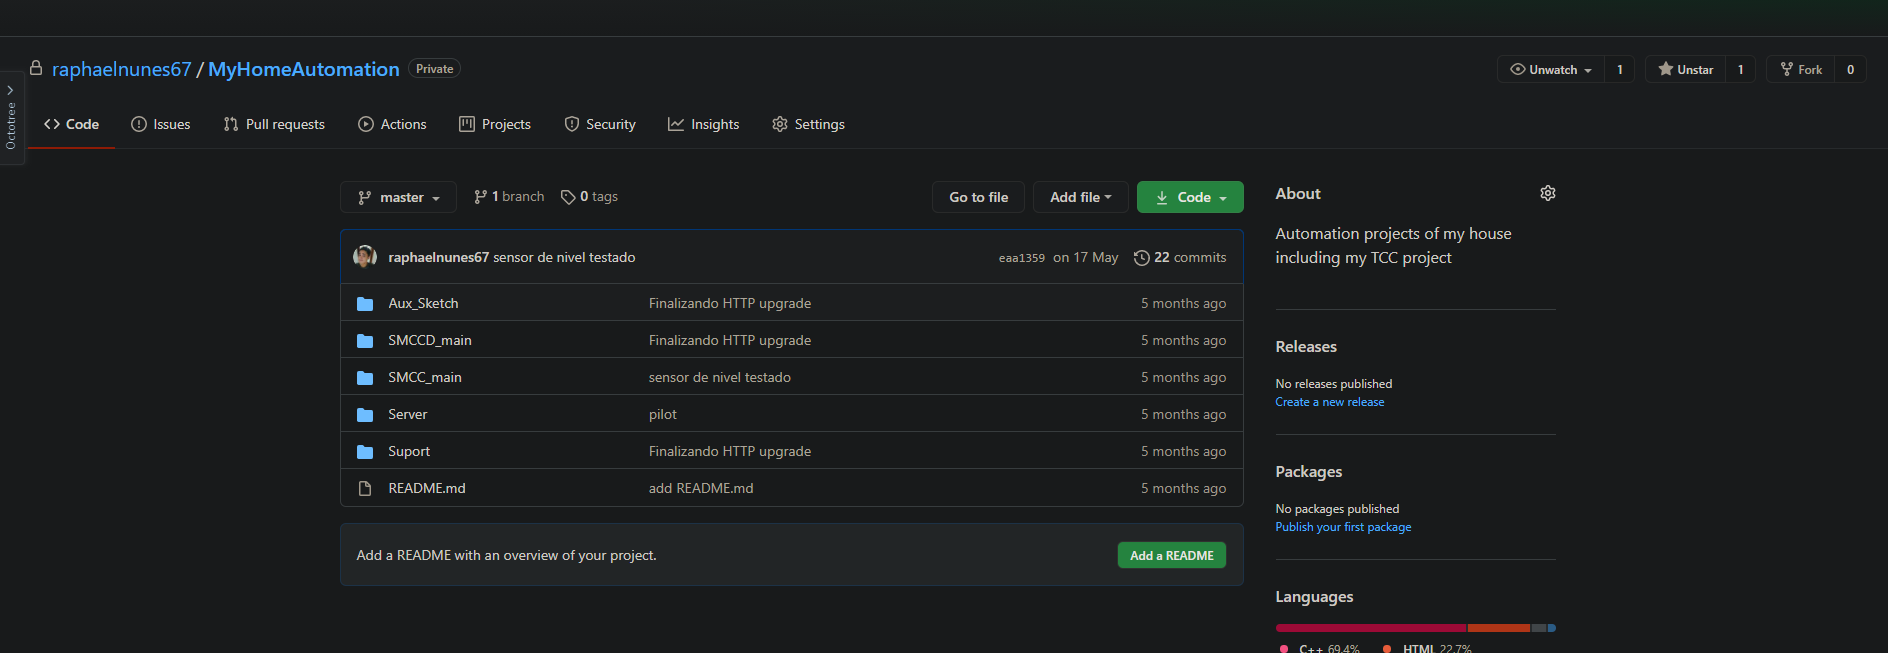
\includegraphics[width=0.85\textwidth]{figuras/github.png}
	\fonte{Própria.}
	\label{fig:github}
\end{figure}

\section{Levantamento do referencial bibliográfico e capacitação}
\label{sec:metmodal}

Essa parte do trabalho conteve-se no levantamento de referências bibliográficas relacionadas com os temas de \textit{IoT}, programação de microcontroladores, criação de aplicações com \textit{frameworks} baseados em \textit{Javascript}. Também buscou-se a capacitação em cursos oferecidos pelas plataformas \textit{Alura}, \textit{Udemy} e \textit{Skylab (Rocketseat)} o aprendizado de conteúdos complementares ao curso de formação em engenheria de controle e automação, como a criação de placas de circuito impresso, treinamentos sobre \textit{Linux} embarcado, implementação do protocolo \textit{MQTT}, criação de \textit{APPs Android} com \textit{React Native} e aplicações \textit{Desktop} com \textit{Electron.js}.

\section{Desenvolvimento dos elementos de \textit{Hardware}}
\label{sec: dev_ele_hardware}

Nesse momento foram definidos todos os elementos de \textit{hardware} necessários para a execução do projeto: para os dispositivos eletrônicos, documentos como \textit{Datasheets}, catálogos e informativos de dispositivos elétricos foram coletados para consulta durante o decorrer do trabalho; para a parte estrutural executou-se a enumeração de peças que deveriam o desenhadas com auxílio do \textit{Software Autodesk Inventor} e posteriormente construídas através de manufatura aditiva.  Realizou-se uma busca no mercado pelos componentes necessários efetuando as possíveis compras e elaborando o orçamento geral do projeto. 

\section{Desenvolvimento dos elementos de \textit{Firmware}}
\label{sec: dev_ele_hardware}

A definição e desenvolvimento dos elementos de \textit{Firmware} se deu após todos os levantamentos de requisitos do trabalho. Esse momento concentrou-se na escolha de tecnologias mais fáceis de implementação, que tivessem uma gama de documentações e que fossem empregadas em produtos oficiais. Para lidar com o uso dos microprocessadores e microcontroladores, foram feitas pesquisas visando consolidar conceitos aprendidos durante o curso de graduação.

\section{Desenvolvimento dos elementos de \textit{Software}}

Para o desenvolvimento dos elementos de \textit{Software} buscou-se a participação de cursos básicos e avançados sobre aplicações \textit{front-end}, as quais servem de conteúdo complementar aos temas abordados na graduação em engenharia de controle e automação.

Os cursos adquiridos trouxeram uma série de conhecimentos para uma maior interação entre desenvolvedor e usuário, possibilitando a criação de interfaces intuitivas e agregando novas informações e visões a outros temas, como na programação de sistemas embarcados.

 
